\documentclass[11pt]{article}
\usepackage[margin=1in]{geometry}
\usepackage{amsmath,amssymb,amsthm,bm}
\usepackage{booktabs,array,longtable}
\usepackage[most]{tcolorbox}
\usepackage{tikz}
\usetikzlibrary{arrows.meta,positioning,shapes.geometric,calc,fit,backgrounds}
\usepackage{hyperref}
\usepackage{xcolor}
\hypersetup{colorlinks=true,linkcolor=blue!50!black,citecolor=blue!50!black,urlcolor=blue!50!black}

% ---- three-level boxes (same house style as doc/algorithms_orbit_transfer.tex)
\newtcolorbox{eli}{colback=green!5,colframe=green!45!black,title=ELI5,fonttitle=\bfseries,breakable}
\newtcolorbox{intu}{colback=blue!4,colframe=blue!45!black,title=Intuition,fonttitle=\bfseries,breakable}
\newtcolorbox{rig}{colback=gray!6,colframe=black!70,title=Rigor,fonttitle=\bfseries,breakable}
\newtcolorbox{warn}{colback=orange!6,colframe=orange!70!black,title=Where it breaks / what is assumed,fonttitle=\bfseries,breakable}
\newtcolorbox{ran}{colback=yellow!6,colframe=yellow!50!black,title=What the script printed,fonttitle=\bfseries,breakable}

\tikzset{
  box/.style={draw,rounded corners,align=center,minimum height=8mm,inner sep=4pt,fill=white,font=\small},
  data/.style={draw,align=center,inner sep=3pt,fill=yellow!12,rounded corners=1pt,font=\scriptsize\ttfamily},
  proc/.style={box,fill=blue!6},
  ext/.style={box,fill=green!8},
  chk/.style={box,fill=orange!8},
  arr/.style={-{Latex[length=2mm]},thick},
  lbl/.style={font=\scriptsize,fill=white,inner sep=1pt}
}

\newcommand{\lv}{\lambda_v}\newcommand{\lr}{\lambda_r}\newcommand{\lm}{\lambda_m}
\newcommand{\tf}{t_f}\newcommand{\R}{\mathbb{R}}
\newcommand{\file}[1]{\texttt{#1}}
\newcommand{\code}[1]{\texttt{#1}}
\newcommand{\Qmt}{Q_{mt}}
\newcommand{\ND}{\mathrm{ND}}

\title{A Guided Reading of \file{transfer\_study.m}\\[2mm]
\large Minimum-time low-thrust transfer from a distant retrograde orbit to a
tulip orbit: the problem, the algorithms, and every condition the script checks}
\author{M.~Casey \quad (Coorbital, \file{orbit\_transfer/DRO\_tulip/})}
\date{2026-09-11}

\begin{document}
\maketitle

\begin{abstract}
\file{transfer\_study.m} solves one low-thrust orbit transfer and then spends
most of its length arguing that the answer is right. This document explains
what it computes and why each line of that argument is there. It is written
for an engineer who knows calculus, differential equations and a little
orbital mechanics, but who has not met Pontryagin's principle, a costate, or
a conjugate point. Everything is said three times: \textbf{ELI5}, a picture in
plain words; \textbf{Intuition}, the reasoning an engineer needs in order to
trust it; \textbf{Rigor}, the equations as the code evaluates them. Where a
result rests on an assumption that could fail, an orange box says so.

The document is self-contained: the optimal control problem, the dynamics, the
two orbits and the maximum principle are all stated here, so the script can be
followed without opening another file. Proofs and the wider library are
elsewhere and are cited where they belong. Every section closes with the
numbers the script actually printed for one run, so the mathematics stays
attached to output the reader can reproduce.
\end{abstract}

\tableofcontents

%=========================================================================
\section{How to read this document}

\file{transfer\_study.m} is a teaching script. It solves a transfer that the
library has already solved, and it does so with the scaffolding deliberately
exposed: the orbits are generated rather than loaded, the boundary conditions
are built in view, the solver is called directly, and each optimality
condition is evaluated and printed on its own line with its own tolerance and
its own verdict. Its companion, \file{build\_70mN\_library.m}, runs the
production chain; this one runs \emph{one} case so that a reader can watch.

The script is organised in ten numbered sections, and so is Part~II of this
document, one section each. Part~I comes first because the script assumes four
things the reader may not have: the problem it is solving, the objects it is
solving it for, what a costate is, and what the maximum principle says. Part~III
closes with what the whole exercise does and does not establish.

\paragraph{The identifier letters.} The script labels its checks. \textbf{N}
is a \emph{necessary} condition of Pontryagin's principle: fail one and the
trajectory is not even a candidate, so nothing below it means anything.
\textbf{S} is a \emph{hypothesis} of the sufficiency theorem --- a hypothesis,
not a conclusion: satisfying S1--S4 together with N1--N6 is what buys the claim
of local optimality. \textbf{V} is a \emph{validity} condition: whether a
verdict above can be believed at all. \textbf{X} is a \emph{cross-check}
against an independent implementation; not a condition of the theory, but a
failure still blocks the claim, because an implementation in doubt cannot
certify anything.

\paragraph{One flight.} The script propagates the converged solution exactly
once, into an object called \code{flight}, and every number in the checking
sections and the figure comes from that object. This is deliberate: a reader
should never have to ask which trajectory owns a reported number.

%=========================================================================
\section{The problem, stated once}\label{sec:ocp}

\begin{eli}
A small spacecraft is parked in one orbit around the Moon and we want it in a
different one. Its engine is feeble --- seventy millinewtons, about the weight
of a strawberry --- so it cannot simply fire once and coast across; it must
thrust almost continuously for weeks, spiralling from one orbit to the other.
Two things are ours to choose at every instant: which way to point the thrust,
and whether the engine is on or off. We want the transfer that takes the least
\emph{time}. The question is what the pointing schedule should be.
\end{eli}

\begin{intu}
Three features make this hard, and each one shows up later as a piece of
machinery.

First, the choice is a \emph{function}, not a number. We are choosing a
pointing direction at every instant of a flight lasting weeks. Calculus of
variations, and its modern form the maximum principle, exists to turn that
infinite-dimensional choice into a finite one.

Second, the dynamics are the three-body problem, which has no closed-form
solution. Everything must be integrated numerically, and the sensitivity of a
weeks-long trajectory to its starting data is severe. That is why so much of
the script is spent measuring residuals.

Third, the final time is \emph{free}. We are not asking for the best transfer
in a given number of days; we are asking for the fastest one, so $\tf$ is
itself an unknown. That single fact is responsible for a surprising amount of
the structure below: it adds one unknown, it supplies one extra condition
($H \equiv 0$), and it forces the second-order test to be done on a quotient
rather than directly.
\end{intu}

\begin{rig}
Work in nondimensional rotating-frame coordinates (\S\ref{sec:cast}). The state
is $x = (r, v, m) \in \R^7$: position, velocity, and mass expressed as a
\emph{fraction} of the initial mass, so $m(0) = 1$. The control is
$u = (\alpha, s)$ with $\alpha \in S^2$ the thrust direction and $s \in [0,1]$
the throttle. The dynamics are
\begin{equation}\label{eq:dyn}
\dot r = v, \qquad
\dot v = g(r) + h(v) + \frac{sT}{m}\,\alpha, \qquad
\dot m = -\frac{sT}{c},
\end{equation}
where $g(r)$ collects the gravity of both primaries and the centrifugal term,
$h(v) = (2v_y, -2v_x, 0)$ is the Coriolis term, $T$ is the thrust acceleration
at unit mass fraction and $c$ the exhaust speed. The minimum-time problem is
\begin{align}
\min_{\alpha(\cdot),\, s(\cdot),\, \tf} \quad & J = \int_0^{\tf} 1 \, dt = \tf
\label{eq:J}\\
\text{subject to} \quad & \eqref{eq:dyn}, \qquad \alpha(t) \in S^2, \quad s(t) \in [0,1], \notag\\
& r(0) = r_0, \quad v(0) = v_0, \quad m(0) = 1, \notag\\
& r(\tf) = r_f, \quad v(\tf) = v_f, \qquad m(\tf) \ \text{free}, \qquad \tf \ \text{free}. \notag
\end{align}
Six conditions are imposed at each end on position and velocity; the terminal
mass is whatever is left. No dry-mass bound is imposed, which is why the
free-mass transversality condition of \S\ref{sec:N4} is unconditional.
\end{rig}

\begin{warn}
Two scope limits that the final verdict must respect. The endpoints
$r_0, v_0, r_f, v_f$ are \emph{fixed points} on the two orbits, chosen by the
phases of \S\ref{sec:sec3}; the problem does not optimise over where on each
orbit to depart and arrive. And the minimum sought is \emph{local}: the whole
apparatus of Part~II establishes that no nearby trajectory does better, not
that no trajectory anywhere does better.
\end{warn}

%=========================================================================
\section{The cast: frame, orbits, phases, engine}\label{sec:cast}

\subsection{The rotating frame and its units}

\begin{eli}
Pick a reference frame that spins with the Moon, so that the Earth and the Moon
both sit still. In that frame the two big bodies are fixed points and only the
spacecraft moves. Then measure distance in Earth--Moon separations and time in
units that make one lunar month equal $2\pi$. Everything becomes a number near
one, which is exactly what a numerical solver wants.
\end{eli}

\begin{intu}
The circular restricted three-body problem (CR3BP) assumes the Earth and Moon
move on a circle about their common barycentre and that the spacecraft is too
light to affect them. In a frame co-rotating with that circle the two primaries
are stationary, and the equations of motion become autonomous --- no explicit
time dependence. Autonomy is not a convenience here; it is load-bearing. It is
precisely why the Hamiltonian is conserved, which in turn is why the free-time
condition takes the clean form $H \equiv 0$ used by check N2.

The price of the rotating frame is the two fictitious terms: centrifugal, which
is folded into $g$, and Coriolis, which is the velocity-dependent $h$.
\end{intu}

\begin{rig}
With $\mu = m_{\text{Moon}}/(m_{\text{Earth}} + m_{\text{Moon}})$, the Earth
sits at $(-\mu, 0, 0)$ and the Moon at $(1-\mu, 0, 0)$. Writing
$d = |r - (-\mu, 0, 0)|$ and $\rho = |r - (1-\mu, 0, 0)|$ for the distances to
Earth and Moon,
\begin{equation}\label{eq:grav}
g(r) = \begin{pmatrix}
x - (1-\mu)\dfrac{x+\mu}{d^3} - \mu\dfrac{x-1+\mu}{\rho^3} \\[2mm]
y - (1-\mu)\dfrac{y}{d^3} - \mu\dfrac{y}{\rho^3} \\[2mm]
- (1-\mu)\dfrac{z}{d^3} - \mu\dfrac{z}{\rho^3}
\end{pmatrix},
\qquad
h(v) = \begin{pmatrix} 2v_y \\ -2v_x \\ 0 \end{pmatrix}.
\end{equation}
The $x$ and $y$ terms outside the fractions are centrifugal. The constants
used throughout are
\[
\mu = 0.012150585609624, \qquad
L^\star = 389\,703.264829278~\text{km}, \qquad
T^\star = 382\,981.289129055~\text{s},
\]
so that one nondimensional time unit is $T^\star \approx 4.43$ days and a
nondimensional period of $2\pi$ is one lunar month.
\end{rig}

\subsection{The departure orbit: a distant retrograde orbit}

\begin{eli}
A distant retrograde orbit, or DRO, is a large loop around the Moon travelled
``backwards'': in the rotating frame the spacecraft circles the Moon in the
opposite sense to the Moon's own motion about the Earth. Backwards turns out to
be remarkably stable. A spacecraft left in a DRO stays there without
station-keeping, which makes it an excellent car park --- somewhere to
accumulate spacecraft cheaply before sending them where they are needed.
\end{eli}

\begin{intu}
The stability is the point. Halo and Lyapunov orbits, the other familiar
cislunar families, are unstable: they sit on saddles, and a spacecraft parked
in one drifts off exponentially unless it is continually corrected. DROs of
moderate size are linearly stable, so the departure end of our transfer is a
place a spacecraft can genuinely wait.

The family is indexed here by its period $\tau$. Larger period means a larger
loop: $\tau = 0.5$ gives a $2.22$-day orbit, $\tau = 1$ a $4.43$-day orbit,
$\tau = 2$ an $8.87$-day orbit. The script takes $\tau = 1$.
\end{intu}

\begin{rig}
The orbit is obtained by natural-parameter continuation onto the periodic
solution of the requested period, then propagated for one period to give a
table $(t_k, r_k, v_k)$. Periodicity is verified as
$|x(\tau) - x(0)| < 10^{-7}$ before anything else runs; a departure orbit that
is not closed is not a departure orbit. The generated table is the raw material
for the endpoint interpolant of \S\ref{sec:sec3}.
\end{rig}

\subsection{The arrival orbit: a tulip}

\begin{eli}
A tulip orbit is a multi-petal orbit around the Moon: the spacecraft traces a
flower-like pattern, coming in close and swinging out again, $N_p$ times per
period, with the far points of the petals concentrated over one lunar
hemisphere. Because the petals hang over one pole, a spacecraft in one spends
a long time high in the sky as seen from that pole --- which is why they are
interesting for navigation and communication at the lunar south pole, where
conventional relay orbits give the weakest coverage.
\end{eli}

\begin{intu}
The essential structural fact, and the one that trips people up, is that the
period of a tulip is \emph{not free}. It is locked to the petal count by a
resonance condition: the orbit must close after $N_p$ petals, which forces
\begin{equation}\label{eq:tulipperiod}
\tau_{\text{tulip}} = 2\pi \, \frac{N_p - 2}{N_p - 1}.
\end{equation}
Choosing $N_p$ therefore chooses the period; there is no separate size knob.
For $N_p = 3, 5, 7, 9$ the periods are $13.93$, $20.89$, $23.21$ and $24.37$
days. The script takes $N_p = 7$, giving $\tau = 2\pi \cdot 5/6 = 5.2360$ and
a $23.21$-day orbit, on the branch $pm = -1$, which is the $z$-mirror of the
other and is the southern one.
\end{intu}

\begin{rig}
As for the DRO: continuation onto the family member, propagation for one
period, and a closure check at $10^{-7}$. The out-of-plane extent
$\max |z|$ is reported because it is the feature that distinguishes the branch
and because a planar result would indicate the wrong family member was
generated.
\end{rig}

\subsection{Phases: where on each orbit}

\begin{eli}
Knowing which two orbits does not yet say where to leave from and where to
arrive. A \emph{phase} is a fraction of the way round an orbit: phase $0$ is
the start of the table, phase $0.25$ is a quarter of a period later. Two phase
numbers, one per orbit, pick the two actual points in space that the transfer
must connect.
\end{eli}

\begin{intu}
The phase pair matters far more than one might expect. At $70$~mN the flight
time across the certified grid varies by roughly fifty percent with the arrival
phase alone. The transfer is not ``DRO to tulip'' as a single number; it is a
two-dimensional sheet of transfers over the departure and arrival phases, and
the script studies one cell of that sheet.

This is also why the endpoints are fixed rather than optimised. Letting the
phases float would be a different and larger problem, with two extra
transversality conditions coupling the costates to the orbit velocities. The
script solves the fixed-phase problem, and its verdict says so explicitly.
\end{intu}

\begin{rig}
A phase $s \in [0,1)$ is converted to a state by evaluating a \emph{periodic
cubic spline} through the propagated orbit table, not by interpolating the
table linearly and not by an ordinary spline. The reason is the seam at
$s = 0$: an ordinary not-a-knot spline is not $C^1$ across it, and a phase near
zero --- which the departure phase is --- is evaluated exactly there. The
shared routine \file{phase\_state} refuses to build anything but a periodic
interpolant unless explicitly asked, and returns its seam mismatch in both
value and derivative for checking.
\end{rig}

\subsection{The engine, and how it becomes two numbers}

\begin{eli}
Three engineering quantities describe the propulsion: how hard it pushes
($70$~mN), how efficiently it uses propellant (specific impulse $900$~s), and
how heavy the spacecraft is to start with ($150$~kg). In the solver's units
these collapse into just two numbers: a thrust acceleration and an exhaust
speed. Everything downstream sees only those two.
\end{eli}

\begin{intu}
The collapse is worth following, because the ratio of those two numbers turns
out to be a safety margin later. Thrust force divided by initial mass is an
acceleration; converting it to nondimensional units gives $T$. Specific impulse
times standard gravity is an exhaust speed; converting gives $c$. The mass
flow is then $\dot m = -sT/c$ per unit initial mass, so $c/T$ is the time it
would take to consume the entire initial mass at full throttle. For this engine
that is $49.4$ nondimensional time units, about $219$ days --- comfortably
longer than the $18$-day transfer, which is why the mass never runs out. The
same ratio reappears in \S\ref{sec:V1} as the threshold of validity condition
H6, for reasons that have nothing to do with running out of propellant.
\end{intu}

\begin{rig}
With $g_0 = 9.80665~\text{m/s}^2$,
\begin{equation}\label{eq:nd}
g_0^{\ND} = g_0 \frac{(T^\star)^2}{1000\,L^\star}, \qquad
c = \frac{I_{sp}}{T^\star} \, g_0^{\ND}, \qquad
T = \frac{F}{m_0} \frac{(T^\star)^2}{1000\, L^\star}.
\end{equation}
For $F = 0.070$~N, $I_{sp} = 900$~s, $m_0 = 150$~kg these give
$T = 1.756418 \times 10^{-1}$ and $c = 8.6737$, hence $c/T = 49.38$.

Because the minimum-time solution turns out to burn continuously
(\S\ref{sec:S2}), the mass obeys a known law for the whole flight:
\begin{equation}\label{eq:masslaw}
m(t) = 1 - \frac{T}{c}\, t,
\end{equation}
which the flight validator checks at every sample rather than only at the end.
\end{rig}

\begin{ran}
\begin{tabular}{@{}lp{0.62\textwidth}@{}}
\toprule
DRO, $\tau = 1$ & period $1.0000$ ND ($4.433$ d), closure $1.19\times10^{-9}$,
  max radius $413\,901$ km\\
Tulip, $N_p = 7$, $pm = -1$ & period $5.2360$ ND ($23.209$ d), closure
  $4.65\times10^{-8}$, $\max|z| = 31\,123$ km\\
Engine & $70$ mN, $I_{sp} = 900$ s, $150$ kg, giving
  $T = 1.756418\times10^{-1}$ and $c = 8.6737$\\
Phases & $s_D = 0$, $s_A = 0.0754$\\
Departure point & $r_0 = (+0.91453,\, +0.00000,\, +0.00000)$\\
Arrival point & $r_f = (+0.97717,\, -0.00184,\, +0.01289)$\\
\bottomrule
\end{tabular}
\end{ran}

%=========================================================================
\section{Costates, and what Pontryagin's principle says}\label{sec:pmp}

This is the section to read twice. Everything the script does after
\S\ref{sec:sec5} is an evaluation of some part of it.

\subsection{The costate}

\begin{eli}
Imagine you are running the transfer and someone offers to nudge your position
slightly, right now, for free. Would you take it? It depends: a nudge in a
helpful direction saves you time later, a nudge in an unhelpful one costs you.
The \emph{costate} is the price list. It is a vector that tells you, at each
instant, how much the remaining cost would change per unit change in each
component of your state. Seven state numbers, seven prices.

The remarkable fact is that if you know the price list at the start, you know
the entire optimal trajectory: the prices obey their own differential equation,
and at every instant the best thing to do is whatever the current prices say is
cheapest. So an infinite-dimensional search over pointing schedules collapses
into a seven-number guess.
\end{eli}

\begin{intu}
The costate $\lambda = (\lr, \lv, \lm)$ is the Lagrange multiplier of the
dynamics constraint, the shadow price of the state. Three features make it
useful rather than merely formal.

It \emph{propagates}. The costate satisfies $\dot\lambda = -\partial H/\partial x$,
an ODE of the same size as the state, integrated alongside it. State and
costate together form a $14$-dimensional system; give it $14$ initial numbers
and everything follows.

It \emph{determines the control}. At each instant the optimal control is the
one minimising a scalar function of the current state and costate. No search
over histories, just a pointwise minimisation, and for this problem that
minimisation has a closed form.

And its velocity part has a name and a meaning. $\lv$ is the \emph{primer
vector}. Its direction is the thrust direction up to sign, and its magnitude is
the sensitivity that tells you whether thrusting is worth anything at all. When
$|\lv| = 0$ the first-order problem stops telling you where to point, and
several things in Part~II break at once; that is why condition S1 exists.
\end{intu}

\begin{rig}
With the normal multiplier normalised to one and the running-cost form
$L \equiv 1$ for minimum time, the Hamiltonian is
\begin{equation}\label{eq:H}
H = 1 + \lr \cdot v + \lv \cdot \big(g(r) + h(v)\big)
+ sT\left(\frac{\lv \cdot \alpha}{m} - \frac{\lm}{c}\right).
\end{equation}
The costate equations $\dot\lambda = -\partial H / \partial x$ are
\begin{equation}\label{eq:costate}
\dot\lr = -\big(\partial_r g\big)^{\!\top} \lv, \qquad
\dot\lv = -\lr - \big(\partial_v h\big)^{\!\top} \lv = -\lr + h(\lv)^{\!\dagger}, \qquad
\dot\lm = \frac{sT}{m^2}\, \lv \cdot \alpha,
\end{equation}
where $\dagger$ denotes the sign flip induced by $h$ being antisymmetric.
Note the structure: $\lr$ is driven by the gravity gradient acting on $\lv$,
and $\lv$ is driven by $\lr$. The mass costate is driven by the thrust term
only.
\end{rig}

\subsection{The control law}

\begin{eli}
The rule turns out to be as simple as it could be. Point the thrust exactly
opposite to the primer vector. Then ask a single number --- call it the switch
function --- whether it is positive: if yes, full throttle; if no, engine off.
For this transfer the number is positive the whole way, so the engine never
stops.
\end{eli}

\begin{intu}
$H$ depends on the direction $\alpha$ only through the inner product
$\lv \cdot \alpha$, which is \emph{linear} in $\alpha$. Minimising a linear
function over the unit sphere is trivial: go to the antipode of the coefficient
vector. That is the entire content of the pointing law, and it is why sampling
the sphere numerically to find the minimiser would test nothing --- the
minimiser is constructed, not found. Condition N6 exists precisely because the
useful question is different: did the \emph{propagator} apply that direction?

$H$ depends on the throttle $s$ linearly too, with coefficient $-T\Qmt$. A
linear function on $[0,1]$ is minimised at an endpoint, which is why the
throttle is bang-bang: full on when the coefficient favours it, off otherwise.
The strict version of that inequality is condition S2, and strictness matters:
if the switch function touched zero, the throttle would be undetermined there
(a singular arc), and the clean structure the whole certification assumes would
be gone.
\end{intu}

\begin{rig}
Over $\alpha \in S^2$, with $\rho := |\lv| > 0$,
\begin{equation}\label{eq:alpha}
\alpha^* = -\frac{\lv}{\rho} \qquad \text{(the primer direction)},
\end{equation}
and substituting, the $\alpha$-minimised Hamiltonian is
$H = 1 + \lr\cdot v + \lv\cdot(g+h) - sT\Qmt$ with the \emph{switch function}
\begin{equation}\label{eq:Q}
\Qmt := \frac{\rho}{m} + \frac{\lm}{c}.
\end{equation}
Hence $s^* = 1$ if $\Qmt > 0$ and $s^* = 0$ if $\Qmt < 0$. With $\alpha^*$
substituted, the mass-costate equation \eqref{eq:costate} becomes
\begin{equation}\label{eq:lammdot}
\dot\lm = -\frac{sT\rho}{m^2} \le 0,
\end{equation}
so $\lm$ is non-increasing --- a fact used three separate times below.
\end{rig}

\subsection{What pins down the seven numbers}

\begin{intu}
Seven initial costates and one final time make eight unknowns. Eight conditions
fix them: six say the trajectory must arrive at the target state in position
and velocity, one is the transversality condition on the free terminal mass,
and one is the free-final-time condition. That is the boundary-value problem
the solver solves, and every one of those eight conditions reappears in Part~II
as something the script re-checks independently.
\end{intu}

\begin{rig}
\textbf{Endpoint conditions.} $r(\tf) = r_f$, $v(\tf) = v_f$: six equations.

\textbf{Free terminal mass} $\Rightarrow$ transversality
\begin{equation}\label{eq:transv}
\lm(\tf) = 0.
\end{equation}
Combined with \eqref{eq:lammdot}, this forces $\lm(t) \ge 0$ along the whole
arc, with $\lm(0)$ its largest value; and since $\rho > 0$ implies $\Qmt > 0$,
the all-burn structure is a \emph{consequence} of the other conditions rather
than an independent assumption. This dependence is stated explicitly in
\S\ref{sec:S2} because it changes what a failure of S2 would mean.

\textbf{Free final time} $\Rightarrow$ $H(\tf) = 0$, and because the system is
autonomous $H$ is conserved, so
\begin{equation}\label{eq:Hzero}
H(t) \equiv 0 \qquad \text{on } [0, \tf].
\end{equation}
This is check N2. Note it is an identity, not a mere constancy: the value is
pinned to zero, and that is what makes it testable.

\textbf{Scaling invariance.} Equations \eqref{eq:alpha} and \eqref{eq:Q} depend
on $(\lr, \lv)$ only through the direction of $\lv$ and, via $\Qmt$, its
magnitude relative to $\lm$. The normalisation $\lambda_0 = 1$ removes the
overall scaling freedom of the multiplier, but the \emph{pair}
$(\lr, \lv) \mapsto (k\lr, k\lv)$ leaves the control law's direction
unchanged. This residual invariance is harmless for the solve and fatal for a
naive second-order test, which is why \S\ref{sec:S4} works on a quotient.
\end{rig}

\begin{warn}
Everything above is \emph{necessary}, not sufficient. A trajectory satisfying
all of it is an \emph{extremal}: a stationary point of the problem. Maxima and
saddles are extremals too. On this very problem, twelve of fourteen candidates
that satisfied every first-order condition were later refuted by the
second-order test of \S\ref{sec:S4}. That is the reason Part~II has a
sufficiency half at all.
\end{warn}

%=========================================================================
\part*{Part II --- The script, section by section}
\addcontentsline{toc}{section}{Part II --- The script, section by section}

\begin{figure}[!h]
\centering
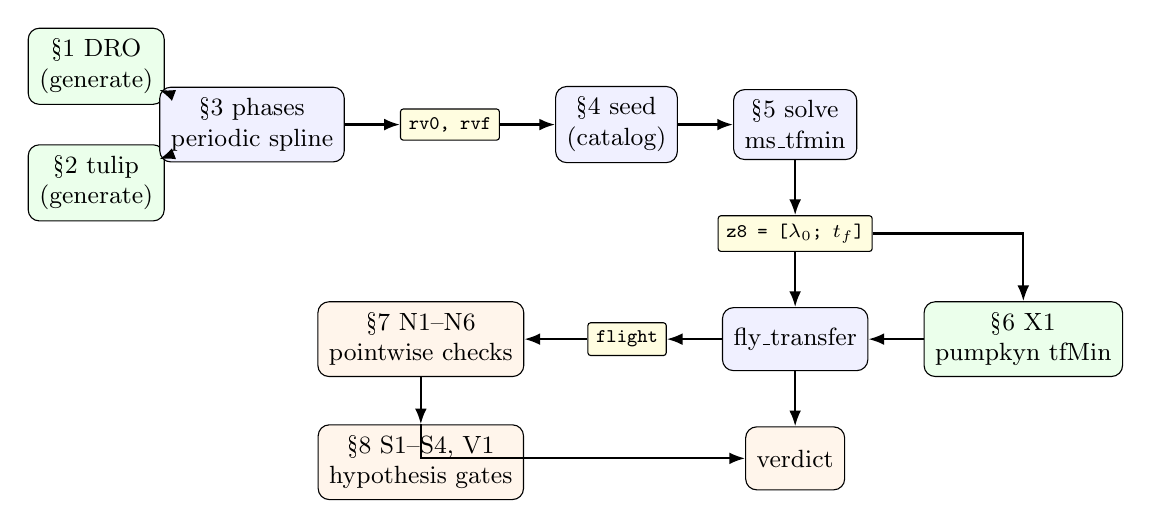
\begin{tikzpicture}[node distance=5mm]
\node[ext] (dro) {\S1 DRO\\(generate)};
\node[ext,below=of dro] (tul) {\S2 tulip\\(generate)};
\node[proc,right=8mm of $(dro)!0.5!(tul)$] (ph) {\S3 phases\\periodic spline};
\node[data,right=7mm of ph] (ends) {rv0, rvf};
\node[proc,right=7mm of ends] (seed) {\S4 seed\\(catalog)};
\node[proc,right=7mm of seed] (solve) {\S5 solve\\ms\_tfmin};
\node[data,below=7mm of solve] (z8) {z8 = [$\lambda_0$; $\tf$]};
\node[proc,below=7mm of z8] (fly) {fly\_transfer};
\node[data,left=7mm of fly] (fl) {flight};
\node[chk,left=8mm of fl] (n) {\S7 N1--N6\\pointwise checks};
\node[chk,below=6mm of n] (s) {\S8 S1--S4, V1\\hypothesis gates};
\node[ext,right=7mm of fly] (x1) {\S6 X1\\pumpkyn tfMin};
\node[chk,below=7mm of fly] (verd) {verdict};
\draw[arr] (dro) -- (ph); \draw[arr] (tul) -- (ph);
\draw[arr] (ph) -- (ends); \draw[arr] (ends) -- (seed);
\draw[arr] (seed) -- (solve); \draw[arr] (solve) -- (z8);
\draw[arr] (z8) -- (fly); \draw[arr] (fly) -- (fl);
\draw[arr] (fl) -- (n); \draw[arr] (n) -- (s);
\draw[arr] (z8) -| (x1); \draw[arr] (x1) -- (fly);
\draw[arr] (s) |- (verd); \draw[arr] (fly) -- (verd);
\end{tikzpicture}
\caption{Data flow of \file{transfer\_study.m}. Green: objects generated or
solved externally. Blue: computation. Orange: checks. Yellow: the data that
passes between them. Note the single \code{flight} object feeding every
check.}
\label{fig:flow}
\end{figure}

%=========================================================================
\section{Section 0: tolerances}\label{sec:sec0}

\begin{eli}
Before anything runs, the script writes down every threshold it will later
judge against, in one place. Not because it is tidy, but because a threshold
written twice eventually gets changed once, and then the report disagrees with
itself.
\end{eli}

\begin{intu}
There is a real methodological point here. A verdict is meaningless without the
tolerance it was measured against, and a tolerance chosen after seeing the
number is not a test. Gathering them at the top, before any computation, makes
both problems visible: every printed line shows value and threshold together,
and the thresholds are committed to in advance.

The tolerances are not all of the same kind, and the document distinguishes
them as it goes. Some are \emph{convergence} tolerances, expressing how well an
equation ought to be satisfied ($10^{-8}$ on the shooting residual). Some are
\emph{screens}, catching gross error rather than certifying precision (the
$100$~km arrival gate). One, the $10^{-7}$ conjugate floor, is an explicit
\emph{policy} value standing in for a measurement not yet made.
\end{intu}

\begin{rig}
The tolerance struct carries: orbit closure $10^{-7}$ and interpolant seam
derivative $10^{-6}$; the shooting residual $10^{-8}$; $|H|$ at $10^{-6}$; the
arrival screens $100$~km and $10$~m/s; transversality $10^{-6}$; the adjoint
relative error $10^{-7}$; the minimum-principle gap $10^{-12}$ and the applied
throttle $10^{-10}$; the cross-check agreement $10^{-6}$; the independent-field
comparison $10^{-10}$; the lift backward error $10^{-6}$ and its Eckart--Young
margin $10\times$; the H6 margin $1\times$; and the instrument agreement
$10^{-6}$.
\end{rig}

%=========================================================================
\section{Sections 1 and 2: generating the two orbits}\label{sec:sec12}

\begin{eli}
The script does not load the two orbits from a file. It builds them from their
defining parameters --- a period for the DRO, a petal count and a branch for the
tulip --- and then checks that what came back actually closes on itself.
\end{eli}

\begin{intu}
Generating rather than loading is a deliberate teaching choice with a real
benefit: the orbits are reproducible from the parameters printed at the top of
the run, so a reader can change one number and see a different transfer. The
closure check is the first assertion in the script because everything
downstream inherits its error. If the departure orbit is closed only to
$10^{-4}$, then the ``periodic orbit'' the transfer departs from is not
periodic at that level, and no amount of precision later recovers it.

Note what closure does \emph{not} check: that the propagation is accurate, or
that the orbit is the intended family member. A wrong-but-closed orbit passes.
The out-of-plane extent is printed for the tulip partly as a guard against
exactly that.
\end{intu}

\begin{rig}
For each orbit: natural-parameter continuation onto the requested member, then
propagation over one period, giving the table used by \S\ref{sec:sec3}. The
assertion is $|x(\tau) - x(0)| < 10^{-7}$ in the full six-vector norm.
\end{rig}

\begin{ran}
DRO: period $1.0000$ ND ($4.433$ d), $105$ samples, closure $1.19\times10^{-9}$.
Tulip: period $5.2360$ ND ($23.209$ d), closure $4.65\times10^{-8}$. Both PASS.
\end{ran}

%=========================================================================
\section{Section 3: engine, phases, endpoints}\label{sec:sec3}

\begin{eli}
Turn the engine's three engineering numbers into the solver's two
(\S\ref{sec:cast}), then convert the two phase fractions into two actual points
in space. The second step sounds trivial and is the one with a subtlety.
\end{eli}

\begin{intu}
The boundary condition the solver matches is not a point on the orbit. It is a
point on an \emph{interpolant} of the orbit table --- and which interpolant is
used is part of the problem definition, not an implementation detail.

Two independent things can go wrong, and the script checks both. The
interpolant might not be smooth where it is evaluated: an ordinary spline has a
kink at the seam $s = 0$, exactly where the departure phase sits. That is why a
periodic cubic is required and why its seam mismatch is reported in value and
derivative. Separately, the interpolant might be smooth but simply wrong ---
sitting off the orbit. Seam smoothness says nothing about that, because a
perfectly periodic interpolant through wrong data is still perfectly periodic.
So the endpoint is also compared against an independent CR3BP propagation to
the same phase. Position and velocity are reported separately, because a
six-vector norm scaled by a length is not a distance.
\end{intu}

\begin{rig}
The seam quantities are the interpolant's value mismatch across $s = 0$ (which
cannot be better than the orbit's own closure) and its derivative mismatch. The
endpoint consistency check propagates the orbit's first sample to $s\tau$ and
compares:
\[
e_r = \big| \text{spline}(s)_{1:3} - r_{\text{prop}} \big|, \qquad
e_v = \big| \text{spline}(s)_{4:6} - v_{\text{prop}} \big|.
\]
This is a consistency estimate against a numerical reference, not a certified
orbit error: it does not establish that the first sample lies on an exactly
periodic orbit, nor bound the reference propagation's own error.
\end{rig}

\begin{ran}
Seam: value $1.2\times10^{-9}$ / $4.6\times10^{-8}$, derivative
$4.5\times10^{-16}$ / $2.3\times10^{-16}$. Interpolant against propagation:
departure $0$, arrival $1.3\times10^{-10}$ ND, which is $0.05$~m in position
and $2.2\times10^{-5}$~m/s in velocity. PASS.
\end{ran}

%=========================================================================
\section{Section 4: the seed}\label{sec:sec4}

\begin{eli}
The solver is Newton's method in disguise, and Newton's method needs a starting
guess. For this problem a guess that is merely ``close'' is not good enough: the
seven costate numbers have no physical intuition attached, they span several
orders of magnitude, and a wrong guess does not converge slowly --- it
converges to something else, or diverges. So the script does not guess. It
looks the answer up in a library of transfers already solved and certified, and
starts from the nearest one.
\end{eli}

\begin{intu}
Why is the guess so hard? Because the map from initial costates to final
position is violently sensitive. The trajectory spirals for weeks; small
changes in the initial primer direction rotate the whole spiral. Measured on
this library, flying from a catalog's recorded $\lambda_0$ missed the target by
tens to hundreds of thousands of kilometres when the recorded control history
landed within ten. The costates are the sensitive object, not the trajectory.

Two consequences shape this section. First, the seed must be a genuinely
converged solution, not an approximation: the library stores certified
entries, one per phase pair on a grid. Second --- and this is the part that
looks like excessive caution until it bites --- the lookup matches the phase
pair \emph{exactly} and refuses anything else. Seeding from a neighbouring
phase is not merely less efficient: a neighbouring phase can lie in the basin
of a \emph{different, slower} branch of the solution family, and that branch
will satisfy every first-order condition the script later checks. It will look
like a perfectly good answer to the wrong question. Refusing by name is
cheaper than discovering that in the verdict.

The seed also carries the operating point, and that is checked in all six
fields: thrust, specific impulse, initial mass, the DRO period, the petal count
and the branch. A seed from a different engine is a seed for a different
problem.
\end{intu}

\begin{rig}
The library holds, per certified phase pair, the converged
$z_8 = [\lambda_0(1{:}7);\, \tf]$ and the multiple-shooting junction states.
The lookup returns a seed structure containing $\tf$, the junction time grid
and the $14 \times (K{+}1)$ junction matrix. When an entry carries only $z_8$,
the junction states are rebuilt by propagating from $z_8$ and slicing. The
certified grid for this operating point is $s_D = k/12$,
$s_A = 0.0754 + j/12$; anything else raises a named refusal.
\end{rig}

\begin{warn}
This is the script's one genuine prerequisite. It studies a transfer the
library has already solved; it is not a tool for finding new ones. Walking to a
new phase pair or a new engine is the job of the continuation front door, and
only after that walk succeeds can the result be studied here.
\end{warn}

\begin{ran}
Seed from the \code{anchor} entry at $(0.0000, 0.0754)$: $24$ segments, its
$\tf = 17.7982$~d; operating point checked in all six fields; $115$ certified
pairs on file.
\end{ran}

%=========================================================================
\section{Section 5: the solve --- multiple shooting}\label{sec:sec5}

\subsection{Shooting, and why once is not enough}

\begin{eli}
Single shooting is the obvious method: guess the seven costates, integrate the
whole flight, see where you land, adjust the guess, repeat. It works for short
flights. For a flight that spirals around the Moon for eighteen days it fails,
because the landing point is so absurdly sensitive to the guess that the
correction step is meaningless --- like trying to hit a target by aiming a rifle
whose barrel amplifies every tremor by a factor of a million.

Multiple shooting cuts the flight into two dozen short pieces. Each piece is
integrated separately, from its own starting state, and we additionally demand
that each piece end where the next one begins. Each individual shot is short, so
each is well behaved. The price is more unknowns; the reward is a problem that
Newton's method can actually solve.
\end{eli}

\begin{intu}
The sensitivity is quantitative, not rhetorical. Sensitivity grows roughly
exponentially with the integration interval, so splitting a flight into $K$
segments replaces one condition number like $e^{\kappa \tf}$ with $K$ of size
$e^{\kappa \tf / K}$. For $\tf$ of eighteen days and $K = 24$ that is the
difference between a Jacobian a solver can factor and one it cannot.

What makes it work as a \emph{method} rather than a trick is that the extra
unknowns come with exactly as many extra equations. Each interior junction
contributes $14$ unknowns (a full state and costate) and $14$ continuity
equations. The count closes, and the solution of the enlarged system, when the
continuity defects are zero, is exactly the solution of the original one.

The structure also buys something the script uses later for free. Newton's
method needs the Jacobian of the residual, and the blocks of that Jacobian are
the state transition matrices of the individual segments --- the derivative of
each segment's endpoint with respect to its start. Those same matrices are what
the conjugate-point test of \S\ref{sec:S4} needs. They are computed anyway, so
the second-order test costs almost nothing extra.
\end{intu}

\begin{rig}
Let $y = (x, \lambda) \in \R^{14}$ be the augmented state and $\varphi(\Delta t, y)$
its flow under \eqref{eq:dyn} with the control law \eqref{eq:alpha},
\eqref{eq:Q} substituted. With $K$ segments on the grid
$0 = t_1 < \cdots < t_{K+1} = \tf$, the unknowns are the junction states
$Y_1, \dots, Y_K$ and $\tf$, where $Y_1$ has its state part fixed to
$(r_0, v_0, 1)$ and only its costate part free. The residual is
\begin{equation}\label{eq:ms}
R = \begin{pmatrix}
\varphi(\Delta t_1, Y_1) - Y_2 \\
\vdots \\
\varphi(\Delta t_{K-1}, Y_{K-1}) - Y_K \\
\Psi\big(\varphi(\Delta t_K, Y_K)\big)
\end{pmatrix},
\end{equation}
where the terminal block $\Psi$ imposes the eight end conditions of
\S\ref{sec:pmp}: $r(\tf) = r_f$, $v(\tf) = v_f$, $\lm(\tf) = 0$, and
$H(\tf) = 0$. The Jacobian $\partial R / \partial(Y, \tf)$ is block
bidiagonal, with the segment state transition matrices
$\Phi_k = \partial \varphi / \partial y$ on the diagonal blocks; it is solved
by a trust-region Newton iteration to $|R|_\infty < 3\times10^{-11}$.
\end{rig}

\begin{warn}
A small residual says the pieces \emph{match each other} and the end conditions
hold. It does not say the pieces are the right equations. A propagator
implementing a wrong control law, or a wrong gravity model, will happily
converge to a self-consistent answer to a different problem --- and the residual
will be just as small. That is the entire reason \S\ref{sec:sec7} exists, and
in particular conditions N5, N6 and X2.
\end{warn}

\subsection{One flight, and its admissibility}

\begin{intu}
With $z_8$ converged, the script propagates once and hands the result to the
same validator the production certifier uses. The check is not ceremony. An
integrator that stops early without throwing returns a short, perfectly finite
trajectory, and every metric taken from its last row then describes a flight
that never happened. So the validator asks: did it reach $\tf$; are the times
real, finite and ordered; are all states and costates finite; does the mass obey
the all-burn law \eqref{eq:masslaw} at \emph{every} sample, not merely the last;
is the expected final mass itself positive; and did the trajectory stay clear of
both primaries.
\end{intu}

\begin{ran}
$11$ Newton iterations, $|R|_\infty = 7.84\times10^{-12}$, converged.
$\tf = 4.015114$ ND $= 17.7976$~d; $\Delta V = 0.7485$~km/s; propellant
$12.20$~kg. Flight: $4193$ samples, admissible; closest approach $6411$~km
(Moon), $332\,599$~km (Earth).
\[
\lambda_0 = (+13.9413,\ +6.26998,\ +7.0227,\ -0.970573,\ -5.0394,\ -3.11587,\ +5.5004).
\]
\end{ran}

%=========================================================================
\section{Section 6: independent verification (X1)}\label{sec:sec6}

\begin{eli}
Hand our answer to somebody else's solver and see whether it wants to change
it. If our seven numbers really solve the problem, a second solver starting
from them has nothing to do. Then, separately, fly \emph{its} answer and check
that it also arrives.
\end{eli}

\begin{intu}
This is not an optimality condition, and the script is careful to report it
apart from the conditions and exclude it from the first-order verdict. It
guards against a different failure: a bug in \emph{our} shooting implementation
producing a self-consistent answer to the wrong problem.

Two halves, because either alone is weak. Agreement alone is not convergence:
a solver that returned its input unchanged on stagnation would report a perfect
zero difference and prove nothing. That possibility was tested directly ---
perturbing the costates by factors of $1.5$, $3$ and $10$ moved the foreign
solver's answer by $9.3$, $37$ and $4612$ --- so it demonstrably does move. And
flying the foreign solution closes the question regardless of that argument:
two independently obtained solutions that both reach the target is a stronger
statement than two vectors that happen to match.
\end{intu}

\begin{warn}
What X1 cannot do is check the physics. Both solvers evaluate the same
equations of motion; a common error in the gravity model, the thrust term or
the mass flow would survive both. This is a cross-check of the
\emph{shooting implementation} on shared dynamics. The independent check of the
physics itself is X2 in the next section.
\end{warn}

\begin{ran}
All eight components agree to $0.00\times10^{0}$; $|dz| = 0$; the foreign
solver's own solution flies to the target within $0.0000$~km and
$0.0000$~m/s. VERIFIED.
\end{ran}

%=========================================================================
\section{Section 7: the necessary conditions}\label{sec:sec7}

Six conditions, evaluated one at a time on the single flight, plus the
independent physics check. Together they establish that the trajectory is an
\emph{extremal}: a stationary point of the problem. They do not establish that
it is a minimum. That is Part~\S\ref{sec:sec8}'s job.

\subsection{N1: the shooting equations are satisfied}\label{sec:N1}

\begin{eli}
Did the solver actually solve its equations? This is the residual it converged
to: how far the pieces are from matching each other and from meeting the end
conditions.
\end{eli}

\begin{intu}
It is tempting to describe N1 as ``the first variation vanishes''. That is the
wrong description, and the script says so. In a problem whose control lives on
a bounded set --- a direction on a sphere, a throttle in $[0,1]$ --- the
first-order condition with respect to the control is not an equation but an
\emph{inequality}: the minimum principle. At full throttle, $H_u = -T\Qmt < 0$,
which is emphatically not zero; what is true is that no \emph{admissible}
variation improves $H$. So N1 is exactly what it is: the PMP shooting
equations, satisfied to tolerance. The control condition is N6.

One subtlety worth carrying: the residual depends on how the arc is propagated.
Measured at this same converged point, requesting the Jacobian (which makes the
integrator carry $210$ states and take finer steps, the mode the solver ran in)
gives $7.84\times10^{-12}$; plain $14$-state propagation gives
$1.41\times10^{-9}$. Both pass the $10^{-8}$ gate, but they differ by $180\times$,
so ``converged to $3\times10^{-11}$'' means ``in the Jacobian mode''. The script
quotes the solver's own number rather than recomputing a different one.
\end{intu}

\begin{rig}
$|R|_\infty$ from \eqref{eq:ms} at the returned point, against $10^{-8}$.
\end{rig}

\subsection{N2: the Hamiltonian vanishes identically}\label{sec:N2}

\begin{eli}
For a problem where the finishing time is free, there is a quantity that must
be exactly zero for the whole flight --- not roughly zero, not constant, zero.
If it drifts, something in the equations is wrong.
\end{eli}

\begin{intu}
Two facts combine. Because the dynamics are autonomous, $H$ is conserved along
any extremal: $dH/dt = 0$. Because the final time is free, the transversality
condition pins its value at the end: $H(\tf) = 0$. Together, $H \equiv 0$.

Why is this a useful test rather than a tautology? Because it is evaluated on
an \emph{independently propagated} flight, using a Hamiltonian assembled from
the state and costate samples, rather than being imposed. Any drift exposes a
defect in the propagation or in the field. What it is \emph{not} is an
independent mathematical restriction: on an exact solution of N1, $H \equiv 0$
follows from $H(\tf) = 0$ plus canonical propagation, and $H(\tf) = 0$ is one of
N1's own equations. The same is true of N4. Both are re-evaluations that catch
numerical defects, not additional reasons to believe the extremal is
minimising.
\end{intu}

\begin{rig}
$\max_k |1 + \lambda_k \cdot f(y_k)|$ over every flight sample, against
$10^{-6}$, with $f$ the $7$-row state field including the mass row.
\end{rig}

\subsection{N3: the flight reaches the target}\label{sec:N3}

\begin{eli}
Fly the converged answer from the start, in one go, and see where it ends up.
\end{eli}

\begin{intu}
This is a \emph{screen}, and the script labels it one. Its tolerances --- $100$~km
and $10$~m/s --- are loose by design, because the quantity being measured is
single-shot propagation error across an eighteen-day arc, which grows with the
arc, not the accuracy of the solution. The fixed-endpoint statement is N1's
residual, which is eleven orders of magnitude tighter. N3's job is to catch
gross error: a solution assembled from the wrong junction states, or flown with
the wrong parameters, misses by thousands of kilometres, and that is what this
line sees.
\end{intu}

\begin{rig}
$|r(\tf) - r_f| L^\star$ in km and $|v(\tf) - v_f| L^\star/T^\star \times 10^3$
in m/s, from the same \code{flight} object as every other number.
\end{rig}

\subsection{N4: transversality on the free mass}\label{sec:N4}

\begin{eli}
Nobody told the spacecraft how much propellant it must have left at the end, so
at the end, propellant is worth nothing. The price of mass must be exactly zero
at the final time.
\end{eli}

\begin{intu}
This is the cleanest instance of what a costate means. $\lm$ is the shadow price
of mass. If the terminal mass is unconstrained and does not appear in the cost,
having a little more of it at the last instant cannot buy anything, so its
price must vanish there. Conversely the price is positive \emph{before} the
end, because mass carried earlier still buys thrust; and by \eqref{eq:lammdot}
it decreases monotonically to its terminal zero.

That monotone decrease is worth holding onto. It means $\lm(0)$ is the largest
value of $\lm$ anywhere on the arc, which is exactly the fact that makes the
validity condition of \S\ref{sec:V1} a single subtraction rather than a search.
\end{intu}

\begin{rig}
$|\lm(\tf)|$ against $10^{-6}$, read from the last flight sample.
\end{rig}

\subsection{N5: the adjoint equations themselves}\label{sec:N5}

\begin{eli}
Check that the price list is obeying its own differential equation --- and check
it against the definition, not against the propagator's own output.
\end{eli}

\begin{intu}
This is where a whole class of bugs hides. The shooting residual says the
pieces match each other; it cannot say the costate equations are the right
ones, because the same wrong equations were used to generate and to match.

So N5 goes back to the definition. It takes the Hamiltonian
\eqref{eq:H} as a function of the state at fixed costate, differentiates it
numerically, and compares with the costate rate the field returns. The
comparison is against $-\partial H/\partial x$ as \emph{defined}, not as
implemented elsewhere.

One practical trap, met and avoided: differencing the propagator's \emph{output}
instead --- taking $(\lambda_{k+1} - \lambda_k)/(t_{k+1} - t_k)$ --- measures the
sample spacing, not the equations. On this arc that approach read
$5\times10^{-4}$, all of it truncation error at the lunar close pass, which
looks like a failure and is not. Differentiating the field at a point, with two
step sizes combined by Richardson extrapolation and their disagreement
reported, is the test that means something.
\end{intu}

\begin{rig}
At $120$ interior samples: central differences of
$\lambda \cdot f(x)$ in each of the seven state coordinates at two step sizes
$h$ and $h/2$, scaled to each coordinate, Richardson-combined as
$(4g_{h/2} - g_h)/3$, compared with $f_{8:14}$ in relative norm against
$10^{-7}$. The two step sizes' disagreement is printed as evidence the
differencing is in its asymptotic regime.
\end{rig}

\subsection{N6: the minimum principle, for the control actually applied}\label{sec:N6}

\begin{eli}
Pontryagin says: at every instant, the control you apply should be the one that
minimises $H$. Checking that by trying lots of directions and seeing which is
best would be pointless here, because we derived the best one in closed form ---
we would only be checking our own algebra. The question worth asking is
different: did the propagator actually \emph{apply} that control? So the check
reaches into the vector field, extracts the control it really used, and measures
how far that is from the optimal one.
\end{eli}

\begin{intu}
Recovering the applied control from the field is the trick that makes this a
real test. The thrust acceleration is the difference between the powered field
and the coasting field, so $b := (m/T)(f_v - f_v^{\,0})$ is the applied
$u\alpha$ --- direction and throttle together. If the propagator's control law
has a sign error, $b$ points the wrong way and the gap opens immediately; a
mutation test injecting exactly that error is part of the test suite, and it
does open the gap, by $5.8$ against a $10^{-12}$ tolerance.

Three refinements matter, each added because its absence was a real hole.
The throttle is recovered on \emph{both} rows it enters, the acceleration rows
and the mass row ($u_{\text{mass}} = -cf_m/T$): the acceleration side alone
cannot see a field that thrusts correctly while consuming mass at half rate,
and a mutation doing precisely that is in the suite. The gap is measured against
the \emph{full} control minimum, direction and throttle, not direction alone.
And its signed minimum is kept, not just the maximum of its absolute value ---
an over-unit thrust aligned with the optimal direction produces a
\emph{negative} gap, which an accumulator starting at zero would have recorded
as a perfect pass.
\end{intu}

\begin{rig}
With $\rho = |\lv|$, $b$ the recovered control, $u = |b|$, and $\Qmt$ from
\eqref{eq:Q}, the gap against the full control minimum is
\begin{equation}\label{eq:gap}
H(u, \alpha) - \min_{\tilde u, \beta} H
= \frac{T}{m}\big(\lv \cdot b + u\rho\big)
+ T\big(\max(\Qmt, 0) - u\,\Qmt\big),
\end{equation}
the first term being the direction part (zero exactly at $b \parallel -\lv$)
and the second the throttle part (zero at $u = 1$ when $\Qmt \ge 0$). The
field's own gap differs from \eqref{eq:gap} by
$(T/c)\lm(u - u_{\text{mass}})$ when the two rows disagree; both are evaluated
and the worse is gated. The weak throttle condition $\Qmt \ge 0$ is reported
here; its strict form is S2.
\end{rig}

\subsection{X2: the physics, against an independent implementation}\label{sec:X2}

\begin{eli}
Every check so far has used the same equations of motion --- the solver's, the
flight's, N2's, N5's. If those equations were wrong in a consistent way, all of
them would agree and all would be wrong. So a second, independently written
version of the dynamics is compared against the first, row by row.
\end{eli}

\begin{intu}
This is the gap X1 does not close. X1 is a second \emph{shooting} implementation
on shared dynamics; X2 is a second \emph{dynamics}. The comparison covers both
halves of the field: the seven state rows against a hand-written CR3BP plus
thrust model, and the seven adjoint rows against the analytic Jacobian of that
model.

The adjoint comparison uses the Jacobian with the control frozen at its applied
value, which deserves a word because it is easy to state wrongly. The envelope
argument says the derivative of the \emph{optimised} Hamiltonian does not pick
up derivatives of the optimising control law --- not that $H_x$ is independent
of the control's value. Here the optimal throttle is locally constant at one
and the optimal direction is state-independent, so the frozen-control
derivative is exact, mass row included:
$\partial f_v/\partial m = -(T/m^2)\alpha$ gives
$\dot\lm = -(T/m^2)\rho$, matching \eqref{eq:lammdot}.
\end{intu}

\begin{rig}
$\max_k |f^{\text{prop}}_{1:7} - f^{\text{ref}}_{1:7}| / \max(1, |f^{\text{ref}}|)$
and the corresponding adjoint-row comparison against
$-A_{\text{ref}}(t)^\top \lambda$, both against $10^{-10}$. These are
vector-norm comparisons of the whole seven-row block, not seven separately
scaled row errors.
\end{rig}

\begin{ran}
\begin{tabular}{@{}llll@{}}
\toprule
ID & quantity & value & threshold \\
\midrule
N1 & $|R|_\infty$ & $7.84\times10^{-12}$ & $10^{-8}$ \\
N2 & $\max|H|$ & $3.32\times10^{-8}$ & $10^{-6}$ \\
N3 & arrival & $0.0000$ km, $0.0000$ m/s & $100$ km, $10$ m/s \\
N4 & $|\lm(\tf)|$ & $7.76\times10^{-10}$ & $10^{-6}$ \\
N5 & adjoint, relative & $3.75\times10^{-10}$ & $10^{-7}$ \\
N6 & $|$full gap$|$ & $9.08\times10^{-15}$ & $10^{-12}$ \\
   & signed extremes & $-9.1\times10^{-15} \ldots +7.5\times10^{-15}$ & \\
   & throttle, acceleration / mass & $5.8\times10^{-15}$ / $0$ & $10^{-10}$ \\
   & $\min \Qmt$ & $3.825$ & $\ge 0$ \\
X1 & second solver $|dz|$ & $0$ & $10^{-6}$ \\
X2 & state rows / adjoint rows & $1.8\times10^{-16}$ / $9.3\times10^{-15}$ & $10^{-10}$ \\
\bottomrule
\end{tabular}
\end{ran}

%=========================================================================
\section{Section 8: the sufficiency hypotheses}\label{sec:sec8}

\begin{intu}
The change of gear here is the most important idea in the script. Everything in
\S\ref{sec:sec7} was \emph{necessary}: any minimum satisfies it. But so does any
maximum, and so does any saddle. The conditions of this section are the
hypotheses of a theorem --- Bonnard--Caillau--Tr\'elat's sufficiency result for
minimum-time problems with free final time --- which, taken together with the
first-order conditions, buys the conclusion that the arc really is a local
minimum.

They are hypotheses, not conclusions. The script's header says so and the
distinction is not pedantic: it determines what a failure means. A failed
necessary condition means the object is not an extremal and nothing else in the
report signifies. A failed sufficiency hypothesis means the theorem does not
apply --- the arc might still be optimal, but this argument no longer shows it.

That these conditions bite is not theoretical. On this problem, twelve of
fourteen candidate solutions that passed every first-order check were refuted by
S4 alone.
\end{intu}

\subsection{S1: the strengthened Legendre condition}\label{sec:S1}

\begin{eli}
At a minimum of an ordinary function the second derivative must be positive, or
you are not at a minimum. The same is true here, but in the control variable:
the Hamiltonian must curve upwards in the thrust direction. It does, and by an
amount proportional to the length of the primer vector --- so the condition
reduces to requiring that the primer never vanishes.
\end{eli}

\begin{intu}
There is an apparent paradox worth resolving, because it catches people. $H$ is
\emph{linear} in $\alpha$, so surely its second derivative is zero?

The resolution is that $\alpha$ is not free in $\R^3$: it lives on the unit
sphere. The relevant second derivative is the one \emph{constrained} to the
sphere --- the Riemannian Hessian --- and a linear function restricted to a
curved surface has genuine curvature. Concretely, moving $\alpha$ along the
sphere away from the minimiser turns it away from $-\lv$, and the penalty is
second order in the angle with coefficient proportional to $|\lv|$. So the
condition is not vacuous, and it degenerates exactly when $|\lv| \to 0$, at
which point the pointing law \eqref{eq:alpha} is undefined anyway.

A vanishing primer would be bad in several ways at once: the direction is
undefined, this Hessian is singular, and the switch function loses its lower
bound. S1 excludes all of that with one number.
\end{intu}

\begin{rig}
For a unit tangent vector to $S^2$ at $\alpha^*$, the constrained second
derivative of $H$ is $uT\rho/m$; at full throttle
\begin{equation}\label{eq:legendre}
H_{\alpha\alpha}\big|_{T_{\alpha^*}S^2} = \frac{T\rho}{m}\, I_2 \succ 0
\iff \rho = |\lv| > 0 .
\end{equation}
The gate is $\min_t |\lv(t)| > 0$ over the propagator's dense samples, with the
location of the minimum reported.
\end{rig}

\subsection{S2: strict bang}\label{sec:S2}

\begin{eli}
The engine must be decisively on, not marginally on. The switch function should
stay strictly positive, with room to spare, rather than grazing zero.
\end{eli}

\begin{intu}
If $\Qmt$ touched zero at an instant, the throttle would be undetermined there:
the linear coefficient vanishes and every throttle value gives the same $H$.
Sustained, that is a \emph{singular arc}, a different and much harder structure
with its own optimality theory. The entire certification here assumes a clean
all-burn bang structure; S2 is the assumption made checkable.

There is an honest dependency to state. On an \emph{exact} lift satisfying
N4, N5 and S1, S2 is not independent of them. Integrating \eqref{eq:lammdot}
backwards from $\lm(\tf) = 0$ gives
\[
\lm(t) = \int_t^{\tf} \frac{u(\sigma) T \rho(\sigma)}{m(\sigma)^2} \, d\sigma \ \ge 0,
\]
so $\rho > 0$ already forces $\Qmt = \rho/m + \lm/c > 0$. S2 therefore cannot
fail while those exact premises hold. Keeping it is still worthwhile: it is a
margin diagnostic, and a failure would tell us that one of the premises is not
in fact established numerically. But it should not be counted as an independent
physical mechanism.
\end{intu}

\begin{rig}
$\min_t \Qmt(t) > 0$ on the dense flight, with the location reported. The weak
version $\Qmt \ge 0$ appears in N6 as a necessary condition; the strict version
is the hypothesis.
\end{rig}

\subsection{S3: normality --- no abnormal lift}\label{sec:S3}

\begin{eli}
There is a degenerate way for a trajectory to satisfy Pontryagin's conditions:
the multiplier on the cost can be zero. Then the conditions say nothing about
minimising anything --- they are satisfied by the constraint geometry alone, and
the ``optimality'' is vacuous. Such a solution is called \emph{abnormal}. S3
checks that our trajectory admits no such degenerate reading.
\end{eli}

\begin{intu}
The maximum principle really has a multiplier $\lambda_0 \ge 0$ in front of the
cost, and $H = \lambda_0 L + \lambda \cdot f$. We set $\lambda_0 = 1$ throughout,
which is a \emph{normalisation}, legitimate only if $\lambda_0 \ne 0$ is
actually the case. An abnormal extremal has $\lambda_0 = 0$: the costates
satisfy all the same equations, but the cost has dropped out entirely.

The test asks a linear-algebra question. Consider all costate histories
compatible with this exact trajectory and this exact control --- the
\emph{lift space} $S$. Each such lift satisfies the adjoint equation with the
control frozen, has its velocity part parallel to the applied thrust direction
at every instant (that is what makes the control optimal for it), and has zero
mass costate at the end. Along any such lift, $\lambda \cdot f$ is conserved, so
it is a linear functional on $S$; its kernel is exactly the abnormal lifts. Our
normal lift has $\lambda \cdot f = -1$, so it is not in the kernel. Therefore if
$S$ is one-dimensional, the kernel is trivial and there is no abnormal lift.

So the hypothesis becomes: $\dim S = 1$.
\end{intu}

\begin{rig}
Stack the constraints over $n$ sample times $t_k$:
\begin{equation}\label{eq:liftC}
C = \begin{bmatrix}
[\alpha(t_1)]_\times \Psi_v(t_1) \\ \vdots \\ [\alpha(t_n)]_\times \Psi_v(t_n) \\
e_m^\top \Psi(\tf)
\end{bmatrix} \in \R^{(3n+1) \times 7},
\qquad \dim S = 7 - \operatorname{rank} C,
\end{equation}
where $\Psi$ is the fundamental matrix of the frozen-control adjoint equation,
$\Psi_v$ its velocity-costate rows, and $[\cdot]_\times$ the cross-product
matrix expressing parallelism. The rank is a numerical judgement, and the
script requires four things rather than one: $\dim S = 1$; the accepted lift's
own \emph{backward error} $|C\lambda_0| / (\|C\| |\lambda_0|)$ small, since a
null space cannot be resolved finer than its known member's residual; the
Hamiltonian residual of the independently assembled field small; and an
Eckart--Young margin, obtained by building $C$ at two integration tolerances
and requiring $\sigma_6$ to exceed the measured difference by a factor.
\end{rig}

\begin{warn}
Two limits of this argument. Eckart--Young with $\sigma_6$ gives
$\operatorname{rank} \ge 6$; rank \emph{exactly} six, and hence $\dim S = 1$,
needs the separately exhibited lift in the kernel, which the normal extremal
supplies only up to its own residual. And the two-tolerance difference is a
sensitivity estimate of one error component --- the adjoint integration --- not
a total error bound: the flown trajectory, its interpolants and the matrix
assembly are common to both builds and cancel in the difference. Finally, the
rank is computed over the whole arc, whereas the theorem's normality hypothesis
is about subarcs; closing that gap by analytic continuation is recorded as open
work.
\end{warn}

\subsection{S4: no conjugate point}\label{sec:S4}

\begin{eli}
Stand at the north pole and walk south along a meridian. For a while, your path
is the shortest route to wherever you have got to. But all meridians meet again
at the south pole --- and once you pass it, your meridian is no longer the
shortest way: you should have gone round the other side. The south pole is a
\emph{conjugate point}: the place where the family of nearby optimal-looking
paths refocuses, and beyond which yours stops being optimal.

The same thing can happen here. The family of nearby trajectories generated by
nudging the initial costates can refocus at some time before arrival. If it
does, the trajectory has stopped being a local minimum at that point, whatever
the first-order conditions say. S4 looks for such a refocusing and finds none.
\end{eli}

\begin{intu}
Concretely: perturb the initial costate and watch how the endpoint moves. That
sensitivity is a matrix, $J(t) = \partial q(t) / \partial p(0)$, the
state-versus-initial-costate block of the state transition matrix. A conjugate
point is a time at which $J$ loses rank: some perturbation of the initial
costates produces \emph{no} change in the state --- the nearby trajectories have
come back together.

Two exact degeneracies must be removed before that rank test means anything,
and forgetting either produces noise determinants of size $10^{-37}$ with
spurious sign flips.

The first is the scaling invariance of \S\ref{sec:pmp}: scaling
$(\lr, \lv)$ leaves the control law unchanged, so that direction produces
identically zero state variation. It is a gauge, not a focus. The columns are
therefore restricted to a complement of it.

The second is the free final time. Variations along the flow direction $f$
merely slide along the same trajectory. In the free-time problem this is a
genuine admissible variation of the endpoint, and appending $f(t)$ as the final
column is what makes the resulting matrix square and its determinant
meaningful. The mass costate is excluded as well, since on an all-burn arc the
control never depends on it and mass is a known function of time.

The determinant is then monitored for sign changes. A sign change strictly
inside $(0, \tf)$ is a conjugate point and refutes the candidate.
\end{intu}

\begin{rig}
With $P$ an orthonormal complement of the scaling direction
$(\lr(0), \lv(0))$, the monitored quantity is
\begin{equation}\label{eq:jacobi}
D(t) = \det \big[\, \Phi_{q\lambda}(t, 0)\, P \ \big|\ f_q(t) \,\big] \in \R^{6\times6},
\end{equation}
sampled at the multiple-shooting junctions, where the segment transition
matrices are already available. Signs are taken from the pivoted LU of the
equilibrated block, magnitudes reassembled as $|D|^{1/6}$ so an underflowing
raw determinant cannot masquerade as an exact zero.
\end{rig}

\paragraph{What the junction test cannot see, and the dense scan.}

\begin{intu}
A sign test at two dozen junctions has two blind spots. Two conjugate times
inside one segment produce two sign changes and hence no net change; and an
even-order zero --- where the determinant touches zero without crossing ---
produces no sign change at all. Both would pass.

So a second instrument samples the singular spectrum densely, eight points per
segment, and treats any dip of the smallest singular value, any trusted
determinant sign change, and any vanishing column as a \emph{candidate} to be
resolved rather than counted. Resolution keeps every evaluation it makes,
re-samples each candidate's window on shifted finer grids, locates every local
minimum by golden section, and then judges the located minimum against a
numerical floor: at or below the floor, or bracketed by opposite trustworthy
signs, it is a zero and the candidate is refuted; a clear factor above the
floor, it is a near miss with a measured positive minimum and is cleared;
anything between is \emph{unresolved} and blocks the claim. Candidates that
touch the very first sample are the structural start-up transient --- the matrix
grows from zero at $t=0$ --- and the interval before the first local maximum is
reported as uncovered rather than cleared.
\end{intu}

\begin{warn}
The floor is a policy value ($10^{-7}$ of the median singular value), standing
in for a measurement of the transition matrix's own accuracy that has not yet
been made. The interval before the first full-rank junction is not covered by
the sign test, and closing it needs a short-time argument rather than more
sampling. Neither instrument encloses roots; both locate and classify.
\end{warn}

\subsection{V1: the validity of the conjugate instrument (H6)}\label{sec:V1}

\begin{eli}
The conjugate test works on a reduced, six-state version of the problem. That
reduction has a booby trap: its determinant can hit zero for a reason that has
nothing to do with a conjugate point, making the instrument cry wolf. There is
a one-line condition that rules the trap out, and it happens to be satisfied
with a factor of nine to spare.
\end{eli}

\begin{intu}
Where does the spurious zero come from? The six-state reduction drops the mass
and its costate, and what remains is \emph{non-autonomous}, because the mass
enters the thrust term as a known function of time. So its reduced Hamiltonian
$h = p \cdot F$ is not conserved. Along the variational equations
$p(t)^\top J(t) = 0$, which means the determinant \eqref{eq:jacobi} carries a
factor of $h(t)$: it can vanish because $h(t) = 0$, not because the rank
dropped. In the full autonomous problem this cannot happen, since $H \equiv 0$
pins things; the reduction loses that protection, and none of the theorem's own
hypotheses covers it.

The saving grace is that $h$ can be computed in closed form. From
$H = 1 + \lambda \cdot f = 0$ and $\dot m = -T/c$,
\[
h = \lambda_{rv} \cdot f_{rv} = -1 + \frac{T}{c} \lm,
\]
which vanishes exactly when $\lm = c/T$. And by N4 and \eqref{eq:lammdot},
$\lm$ decreases monotonically from $\lm(0)$ to zero. So its largest value on
the whole arc is $\lm(0)$, and the mechanism cannot fire if and only if
$\lm(0) < c/T$. One subtraction, computable for every catalog entry.

This is where $c/T$ returns. It arrived in \S\ref{sec:cast} as the time to
consume all the propellant; it reappears here as a threshold on the initial
price of mass, for entirely unrelated reasons.
\end{intu}

\begin{rig}
\begin{equation}\label{eq:H6}
\text{H6:} \qquad \lm(0) < \frac{c}{T},
\end{equation}
gated as the helper's own verdict --- a strict margin \emph{and} a clearance of
$h_{\max} = -1 + (T/c)\lm(0)$ below zero by more than the arc's Hamiltonian
residual, since the reduced Hamiltonian is known no better than that.
Equivalently, by $\int_0^{\tf} T\Qmt \, dt = \lm(0)$, the condition says the
total strict-bang margin stays below $c/T$.
\end{rig}

\begin{warn}
H6 is a statement about this normalisation. With a general objective multiplier
$p_0$ the threshold reads $\lm(0) < (c/T) p_0$; it is correct here because the
solver fixes $p_0 = 1$.
\end{warn}

\subsection{V2: the wiring check}\label{sec:V2}

\begin{intu}
The two instruments --- the pointwise checks, which read the flight the script
flew, and the hypothesis gates, which fly their own from $z_8$ --- are compared
on the switch function's minimum. They agree to exactly zero, because both
propagate the same $z_8$ deterministically, and the script says so rather than
presenting the agreement as evidence.

What it can catch is the mistake that actually happens when a section is
edited: handing one instrument the wrong flight or the wrong exhaust speed.
What it cannot catch, and the script now says this too, is a wrong thrust or
mass ratio, because $\Qmt$ is computed from the flight samples and $c$ alone.
Those surface in N2 instead.
\end{intu}

\subsection{The verdict}\label{sec:verdict}

\begin{intu}
The script's closing statement has four possible outcomes, and the distinctions
are the point: a claim; not an extremal, in which case nothing second-order is
even meaningful; unresolved, in which case nothing is claimed \emph{and} nothing
is refuted; or an extremal whose sufficiency fails.

When it claims, it claims carefully. It names the exact problem: fixed
departure and arrival position and velocity, initial mass fraction one, free
terminal mass and free final time, with the phases fixed inputs rather than
optimised quantities. It states that the evidence is numerical and sampled,
with no between-sample bounds, that $\dim S$ is a numerical rank with a measured
rather than proven error, and that the conjugate scan locates and clears
candidates against a floor rather than enclosing roots. And it names the three
structural conditions that the diagnostics do not establish at all: the subarc
normality argument, the reduction of the free-mass free-time second variation to
the six-state problem, and the existence of an exact extremal near the numerical
one.
\end{intu}

\begin{ran}
\begin{tabular}{@{}lll@{}}
\toprule
ID & quantity & value \\
\midrule
S1 & $\min|\lv|$ & $3.2359$ at $t/\tf = 0.117$ \\
S2 & $\min \Qmt$ & $3.8248$ at $t/\tf = 0.984$ \\
S3 & $\dim S$ & $1$ \\
   & lift backward error & $5.3\times10^{-10}$ (threshold $10^{-6}$) \\
   & $|\lambda \cdot f + 1|$ & $3.3\times10^{-8}$ \\
   & Eckart--Young margin & $2545\times$ ($\sigma_6 = 0.678$ vs $|dC| = 2.66\times10^{-4}$) \\
S4 & junction sign test & PASS, $0$ crossings, $\min|D| = 2.43\times10^{-4}$ \\
   & coverage & $24$ junctions, first full rank $t/\tf = 0.042$, through $\tf$ \\
   & identities & $Jp(0) = 0$ to $3.8\times10^{-15}$; $p^\top J = 0$ to $8.0\times10^{-14}$ \\
   & dense scan & $192$ samples, $2$ candidates, both near-miss; $0$ zero, $0$ unresolved \\
V1 & $\lm(0)$ vs $c/T$ & $5.500$ vs $49.383$, margin $9.0\times$, clearance $0.889$ \\
V2 & instrument agreement & $0$ \\
\bottomrule
\end{tabular}
\end{ran}

%=========================================================================
\section{Section 9: the figure}\label{sec:sec9}

The script closes by drawing the transfer in three dimensions --- both orbits,
the flown arc, the two endpoints --- from the same \code{flight} object that
produced every number above. It is rotatable, which matters more than it
sounds: the out-of-plane structure of the tulip and the way the transfer climbs
into it are not legible in a fixed projection.

%=========================================================================
\part*{Part III --- What this establishes}
\addcontentsline{toc}{section}{Part III --- What this establishes}

\section{Proven, assessed, assumed}\label{sec:proves}

\begin{intu}
It is worth separating three very different kinds of statement that the script
prints in the same format, one line each with a PASS at the end.

\textbf{Proven, given the numbers.} Some conditions are exact algebraic
consequences of quantities we computed. If $\min|\lv| = 3.24$ at every sampled
time then the Legendre form is positive definite at those times; there is no
inference gap, only a sampling one.

\textbf{Assessed numerically.} Most of the report is of this kind. $\dim S = 1$
is a numerical rank with a measured, not proven, error. The conjugate verdict
is a sign test at junctions plus a located-minimum scan, neither of which
encloses a root. The residuals are evaluated at samples with no bound between
them. These are strong evidence and not certificates, and the distinction is
not academic: a genuine even-order zero between two samples would be invisible
to a sign test, which is exactly why the second instrument exists.

\textbf{Assumed, and named.} Three structural items are not addressed by any
diagnostic: that the whole-arc normality computed in S3 implies the subarc
condition the theorem actually requires; that the free-mass, free-time second
variation reduces to the six-state problem the conjugate determinant tests; and
that an exact extremal exists near the numerical one, which no residual alone
can supply. The verdict names all three.
\end{intu}

\begin{rig}
\begin{tabular}{@{}p{0.30\textwidth}p{0.62\textwidth}@{}}
\toprule
Claim & Status \\
\midrule
The arc is an extremal & Assessed: N1--N6 at tolerance, on sampled times, with the physics independently checked (X2) and the shooting independently reproduced (X1) \\
The control is the PMP control & Assessed exactly at $120$ interior samples, on both rows the control enters \\
No abnormal lift & Assessed: rank six with an Eckart--Young margin of $2545\times$ against a \emph{sensitivity} estimate of one error component \\
No conjugate point in $(0,\tf]$ & Assessed: no sign change at $24$ junctions, no located zero on $192$ dense samples; the interval before $t/\tf = 0.042$ is uncovered \\
The instrument is valid & Proven given $\lm(0)$: H6 holds with a $9\times$ margin and a clearance above the Hamiltonian residual \\
Strict strong local minimum & Conditional: follows from the theorem \emph{if} the three assumed items hold and the sampled evidence reflects the continuum \\
\bottomrule
\end{tabular}
\end{rig}

\section{Open items}\label{sec:open}

These are recorded in \file{costate\_common/TODO.md} and are the honest edge of
the argument.

\begin{enumerate}
\item \textbf{Subarc normality.} Establish that every relevant subarc has the
normality the theorem requires, by analytic continuation of the strict all-burn
extremal. The terminal condition $\lm(\tf) = 0$ does not transfer to a moved
subarc endpoint unchanged, and the argument must say where H6 supplies the
necessary normalisation.

\item \textbf{The six-state reduction.} Write the reduction of the free-mass,
free-time second variation and critical cone to the six-state non-autonomous
problem, covering the competitor class --- including reduced-throttle
directions --- so the claim remains \emph{strong} local rather than restricted.

\item \textbf{The uncovered initial interval.} A short-time expansion
establishing non-conjugacy and a definite determinant sign on some
$(0, \varepsilon]$, overlapping the tested region.

\item \textbf{Between-sample bounds.} Derivative bounds or interval integration
for $|\lv| > 0$, $\Qmt > 0$, the primary clearances, and the conjugate matrix
itself.

\item \textbf{A measured floor.} The conjugate scan's zero floor and the
sign-trust threshold are policy values. Both should come from a measured error
in the scaled matrix at the candidate times, obtained by re-propagating from
$t = 0$ at a tighter setting or with a different integrator.

\item \textbf{Existence of a nearby exact extremal.} A validated shooting solve
or a Newton--Kantorovich argument; a small residual does not supply it.
\end{enumerate}

\section*{Glossary}
\addcontentsline{toc}{section}{Glossary}

\begin{description}
\item[Abnormal extremal] One whose cost multiplier $\lambda_0$ is zero, so the
PMP conditions carry no information about minimising the cost. Excluded by S3.
\item[Bang-bang] A control that takes only its extreme values. Here the
throttle is $1$ throughout (all-burn), because the switch function stays
positive.
\item[Conjugate point] A time at which the family of nearby extremals refocuses
and the arc stops being locally minimising; the south pole of the meridian
picture in \S\ref{sec:S4}.
\item[Costate] The vector of shadow prices $\lambda = (\lr, \lv, \lm)$, the
sensitivity of the remaining cost to the state.
\item[DRO] Distant retrograde orbit: a large, linearly stable, retrograde loop
about the Moon in the rotating frame.
\item[Extremal] A trajectory satisfying the first-order PMP conditions. Minima,
maxima and saddles are all extremals.
\item[Lift] A costate history compatible with a given trajectory and control.
The set of them is the lift space $S$ of S3.
\item[Multiple shooting] Solving a boundary-value problem by cutting the
interval into segments, integrating each separately, and imposing continuity.
\item[Primer vector] The velocity costate $\lv$; its direction gives the
optimal thrust direction, its magnitude the sensitivity to thrusting.
\item[Seed] A converged solution used as the starting guess for a nearby one.
\item[Switch function] $\Qmt = |\lv|/m + \lm/c$; its sign decides the throttle.
\item[Transversality] The endpoint conditions the multipliers must satisfy;
here $\lm(\tf) = 0$ from free terminal mass and $H(\tf) = 0$ from free final
time.
\item[Tulip orbit] A multi-petal cislunar periodic orbit whose period is locked
to its petal count by \eqref{eq:tulipperiod}.
\end{description}

\section*{Where to go next}
\addcontentsline{toc}{section}{Where to go next}

\begin{description}
\item[\file{doc/algorithms\_orbit\_transfer.tex}] The library-wide algorithmic
reference: the same optimal control problem for three objectives, the min-time
and min-fuel pipelines end to end, and the data model.
\item[\file{DRO\_tulip/doc/dro\_tulip\_mintime.tex}] The same transfer from the
\emph{direct} side: collocation, Hermite--Simpson, path constraints, IPOPT, and
the lessons that produced the current formulation.
\item[\file{doc/mintime\_second\_order\_audit.tex}] The proof that the
instrument's quotiented determinant is the Bonnard--Caillau--Tr\'elat test, the
two exact reductions it rests on, and what a PASS means.
\item[\file{doc/bct\_hypothesis\_dictionary.tex}] The sufficiency theorem
written as a dictionary from its hypotheses to this problem's quantities.
\item[\file{DRO\_tulip/FINDINGS.md}] The running record, including the three
external reviews of this script and what each one changed.
\end{description}

\section*{References}
\addcontentsline{toc}{section}{References}

\begin{enumerate}
\item L.~S.~Pontryagin, V.~G.~Boltyanskii, R.~V.~Gamkrelidze, E.~F.~Mishchenko,
\emph{The Mathematical Theory of Optimal Processes}, Interscience, 1962.
\item B.~Bonnard, J.-B.~Caillau, E.~Tr\'elat, ``Second order optimality
conditions in the smooth case and applications in optimal control'',
\emph{ESAIM: COCV} 13(2), 2007.
\item J.-B.~Caillau, O.~Cots, J.~Gergaud, ``Differential continuation for
regular optimal control problems'', \emph{Optimization Methods and Software}
27(2), 2012.
\item A.~V.~Sarychev, ``The index of second variation of a control system'',
\emph{Mat.~Sbornik} 41, 1982.
\item J.~T.~Betts, \emph{Practical Methods for Optimal Control Using Nonlinear
Programming}, 3rd ed., SIAM, 2020, ch.~3 (multiple shooting).
\item D.~Koblick, M.~Casey, ``A Tulip-Orbit Constellation for Lunar South-Pole
Navigation and Direct-to-Earth Relay'', arXiv:2607.10482, 2026.
\end{enumerate}

\end{document}
